\documentclass[conference]{IEEEtran}
\IEEEoverridecommandlockouts

% ===================== Packages =====================
\usepackage{cite}
\usepackage{amsmath,amssymb,amsfonts}
\usepackage{algorithmic}
\usepackage{graphicx}
\usepackage{textcomp}
\usepackage{xcolor}
\usepackage{booktabs}
\usepackage{array}
\usepackage[caption=false,font=footnotesize]{subfig}
\usepackage{placeins}

% Tighter float spacing for two-column report
\setlength{\textfloatsep}{6pt plus 1pt minus 2pt}
\setlength{\floatsep}{5pt plus 1pt minus 2pt}
\setlength{\intextsep}{6pt plus 1pt minus 2pt}
\renewcommand{\topfraction}{0.95}
\renewcommand{\dbltopfraction}{0.95}
\renewcommand{\floatpagefraction}{0.85}
\renewcommand{\dblfloatpagefraction}{0.85}

% ===================== Title / Authors =====================
\title{COMP0222 Coursework 02: Visual and LiDAR SLAM}

\author{
\IEEEauthorblockN{Group Code: TODO}
\IEEEauthorblockA{
Department of Computer Science\\
University College London\\
London, United Kingdom}
}

\begin{document}
\maketitle

% ===================== Abstract =====================
\begin{abstract}
This report presents our experiments for COMP0222 Coursework 02. We evaluate visual SLAM on public datasets and on self-collected monocular sequences, and we evaluate 2D LiDAR SLAM on self-collected laser scans. For the self-collected visual SLAM task, we acquire one indoor and one outdoor RGB sequence, reconstruct them with COLMAP, track them with monocular ORB-SLAM2, and compare the estimated camera trajectories using EVO. For the LiDAR task, we analyse laser odometry, mapping, loop closure detection, and factor graph optimisation.
\end{abstract}

\begin{IEEEkeywords}
Visual SLAM, LiDAR SLAM, ORB-SLAM2, COLMAP, EVO, monocular camera, trajectory evaluation
\end{IEEEkeywords}

% ============================================================
\section{Visual SLAM with Public Datasets}
\label{sec:q1_public_datasets}

% TODO: Insert Question 1 content here.
% Suggested structure:
% \subsection{Dataset Description}
% \subsection{Baseline Evaluation}
% \subsection{Effect of ORB Feature Number}
% \subsection{Effect of Outlier Rejection}
% \subsection{Effect of Loop Closure}
% \subsection{Discussion}

This section is reserved for Question 1. It should include the KITTI 07 and TUM monocular ORB-SLAM2 experiments, the EVO evaluation plots, the tested parameter settings, and a discussion of how ORB feature number, outlier rejection, and loop closure affect trajectory quality.

% ============================================================
\section{Visual SLAM with Our Own Sequences}
\label{sec:q2_visual_slam}

\subsection{Overview}

For Question 2, we collected two monocular RGB video streams: one indoor sequence and one outdoor sequence. Both were captured as continuous image streams rather than disconnected still images. We used COLMAP for camera calibration refinement, sparse reconstruction, and camera trajectory extraction. The same sequences were then tracked using monocular ORB-SLAM2 with fixed RealSense D455 calibration. Finally, EVO was used to compare the ORB-SLAM2 trajectories against the refined COLMAP trajectories.

Since no external motion-capture, LiDAR, or survey-grade ground truth was available for these self-collected sequences, the EVO results should be interpreted as agreement with COLMAP rather than absolute metric accuracy. Sim(3) alignment was used because both COLMAP and ORB-SLAM2 are monocular pipelines and therefore have arbitrary global scale.

\subsection{Data Collection and Calibration}

\subsubsection{Acquisition Strategy}

The data were collected using the colour stream of an Intel RealSense D455 camera at $848 \times 480$ resolution and 30 FPS. During capture, the camera was hand-carried at approximately constant height and moved slowly through each environment. We deliberately used translational motion rather than pure yaw rotation, because monocular reconstruction requires parallax for reliable triangulation. Sudden turns were avoided where possible to reduce motion blur and preserve feature overlap between consecutive frames.

The indoor sequence, \textit{indoor\_02}, was captured in a large office/atrium area containing tables, chairs, white walls, glass doors, carpet, repeated planar structures, and occasional people. The outdoor sequence, \textit{outdoor\_01}, was captured in a covered courtyard/walkway with tables, poles, barriers, signs, glass facades, and building edges. Representative frames are shown in Fig.~\ref{fig:q2_raw_frames}.

\begin{figure}[!t]
\centering
\subfloat[Indoor.]{
    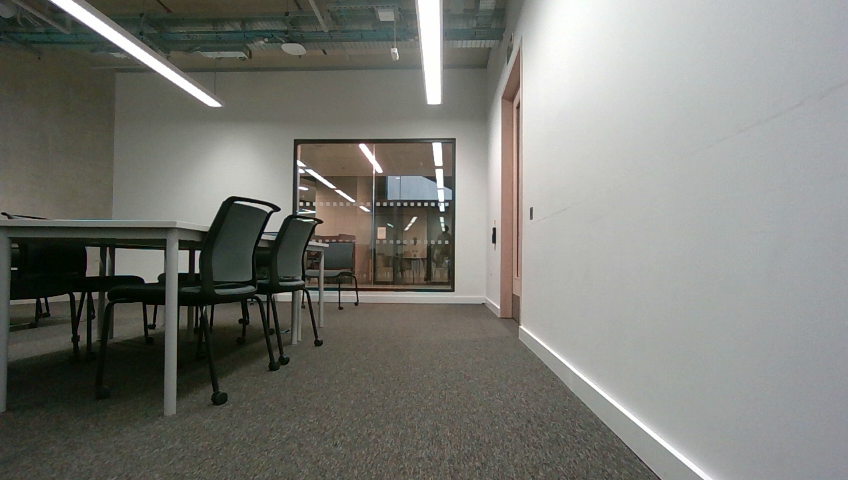
\includegraphics[width=0.48\linewidth]{images/Q2/figures/raw_frames/indoor_000000.png}
}
\hfill
\subfloat[Indoor.]{
    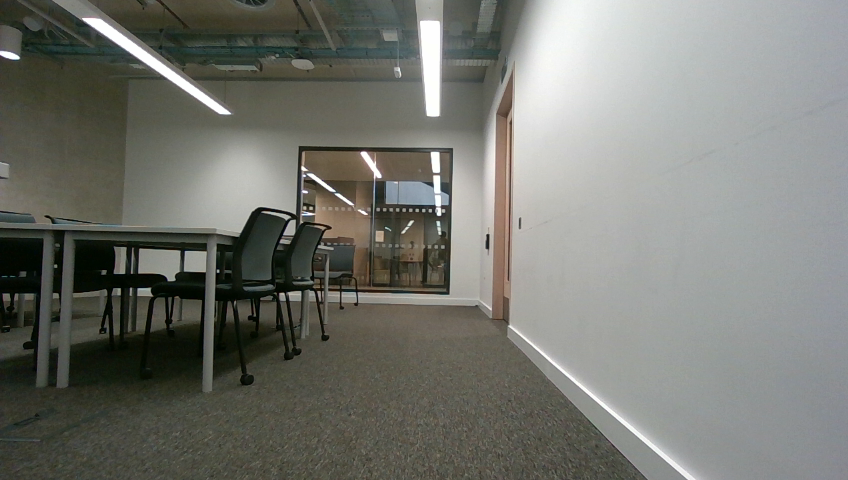
\includegraphics[width=0.48\linewidth]{images/Q2/figures/raw_frames/indoor_001242.png}
}

\vspace{1mm}

\subfloat[Outdoor.]{
    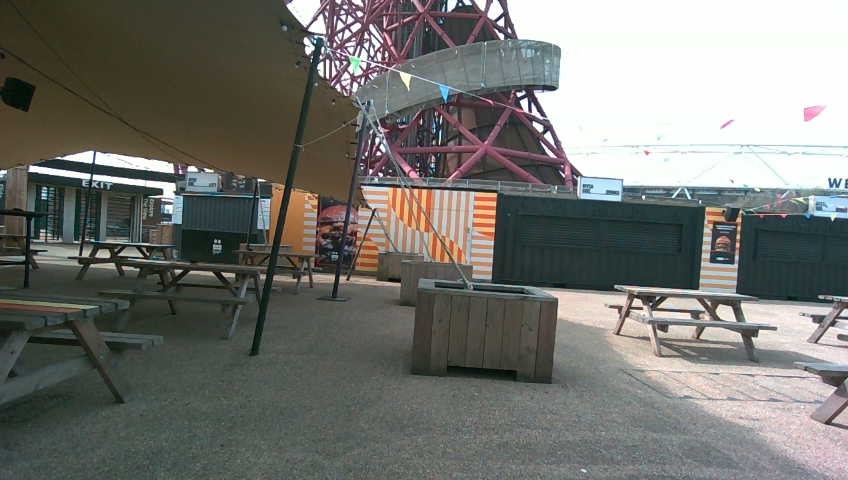
\includegraphics[width=0.48\linewidth]{images/Q2/figures/raw_frames/outdoor_000000.png}
}
\hfill
\subfloat[Outdoor.]{
    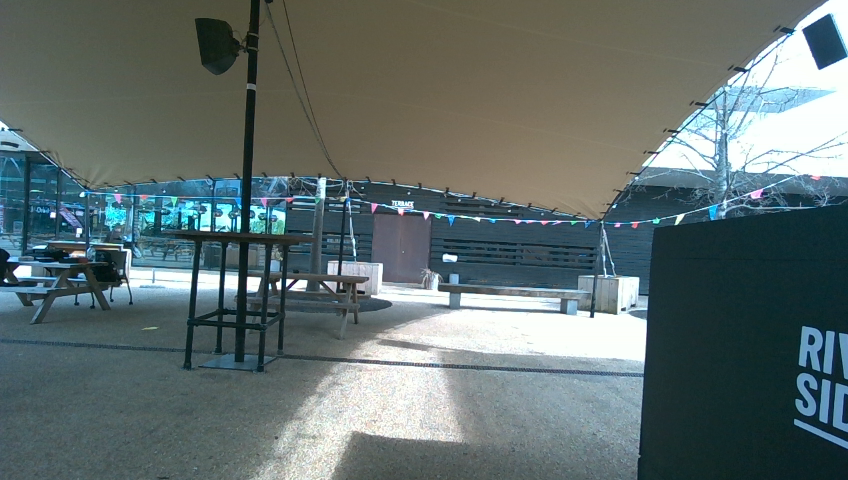
\includegraphics[width=0.48\linewidth]{images/Q2/figures/raw_frames/outdoor_002119.png}
}
\caption{Representative frames from the self-collected monocular streams. The indoor sequence contains larger low-texture planar regions, while the outdoor sequence provides stronger geometric edges and more stable visual structure.}
\label{fig:q2_raw_frames}
\end{figure}

Table~\ref{tab:q2_sequence_stats} summarises the capture and image-quality statistics. Both sequences contain more than 500 frames after ORB-SLAM2 initialisation. The outdoor sequence has much higher Laplacian blur variance and more good inter-frame matches, indicating sharper images and more stable feature correspondences.

\begin{table}[!t]
\caption{Capture and processing statistics for the self-collected monocular sequences. Blur is measured using Laplacian variance; brightness is mean grey value.}
\centering
\footnotesize
\begin{tabular}{lcc}
\toprule
Quantity & Indoor & Outdoor \\
\midrule
Resolution & \multicolumn{2}{c}{$848 \times 480$} \\
Frame rate & \multicolumn{2}{c}{30 FPS} \\
Raw frames & 2222 & 3275 \\
Duration (s) & 74.1 & 109.1 \\
COLMAP sampled images & 600 & 600 \\
COLMAP registered images & 600 & 600 \\
ORB-SLAM2 input frames & 2218 & 3269 \\
Frames after initialisation & $>$500 & $>$500 \\
Mean blur & 301.8 & 1049.5 \\
Mean brightness & 116.8 & 109.9 \\
Mean ORB features & 1099.0 & 1200.0 \\
Mean good matches & 259.9 & 425.9 \\
\bottomrule
\end{tabular}
\label{tab:q2_sequence_stats}
\end{table}

\subsubsection{Calibration and Processing Settings}

The RealSense SDK factory intrinsics were read at the capture resolution and used as the fixed ORB-SLAM2 calibration. COLMAP used a shared FULL OPENCV camera model initialised from the D455 intrinsics and refined it during bundle adjustment. The refined focal lengths remained close to the factory values: indoor $f_x = 429.677$, $f_y = 429.681$; outdoor $f_x = 428.907$, $f_y = 428.471$. The final bundle-adjustment costs were 0.517 px for indoor and 0.425 px for outdoor, supporting the validity of the initial calibration.

ORB-SLAM2 was run in monocular mode on the full filtered streams. Loop closing and outlier rejection were kept enabled. The configuration used 2000 ORB features, scale factor 1.2, 8 pyramid levels, and FAST thresholds 20/7. The camera parameters used in the ORB-SLAM2 YAML file are shown in Table~\ref{tab:q2_orbslam_yaml}.

\begin{table}[!t]
\caption{ORB-SLAM2 monocular configuration used for both self-collected sequences.}
\centering
\footnotesize
\begin{tabular}{lc}
\toprule
YAML parameter & Value \\
\midrule
Camera.fx & 426.7957 \\
Camera.fy & 426.2545 \\
Camera.cx & 427.2596 \\
Camera.cy & 250.0979 \\
Camera.k1 & -0.05605 \\
Camera.k2 & 0.06574 \\
Camera.p1 & -0.000917 \\
Camera.p2 & 0.000815 \\
Camera.k3 & -0.02142 \\
Camera.fps & 30 \\
ORBextractor.nFeatures & 2000 \\
ORBextractor.scaleFactor & 1.2 \\
ORBextractor.nLevels & 8 \\
FAST thresholds & 20 / 7 \\
\bottomrule
\end{tabular}
\label{tab:q2_orbslam_yaml}
\end{table}

COLMAP was run on sampled image streams to keep reconstruction tractable while preserving route coverage. We used every 3rd frame for the indoor stream and every 5th frame for the longer outdoor stream, capped at 600 images per sequence. Sequential matching was used because the data were captured as ordered video streams. The sparse COLMAP model was used for trajectory extraction because COLMAP estimates camera poses during sparse structure-from-motion and bundle adjustment. Dense reconstruction was not used for trajectory evaluation.

\subsection{Indoor Sequence}

The indoor sequence was successfully reconstructed and tracked, but it was the more challenging case. COLMAP registered all 600 sampled images and recovered the overall loop-like route. However, the scene contains white walls, glass, carpet, repeated planar structures, and occasional moving people. These factors reduce distinctive long-term feature tracks and can create ambiguous feature matches.

Fig.~\ref{fig:q2_indoor_summary} summarises the indoor result. The COLMAP sparse model is valid for trajectory extraction because all sampled images were registered and the global route structure was recovered. ORB-SLAM2 also produced a coherent sparse map and exported 158 keyframes with 10,859 sparse map points. The EVO comparison shows that the ORB-SLAM2 trajectory follows the same route as COLMAP, but with larger local deviations around weak-texture and repeated-structure regions. The indoor APE RMSE is 0.1221 and the RPE RMSE is 0.0281.

\begin{figure*}[!t]
\centering
\subfloat[COLMAP sparse top view.]{
    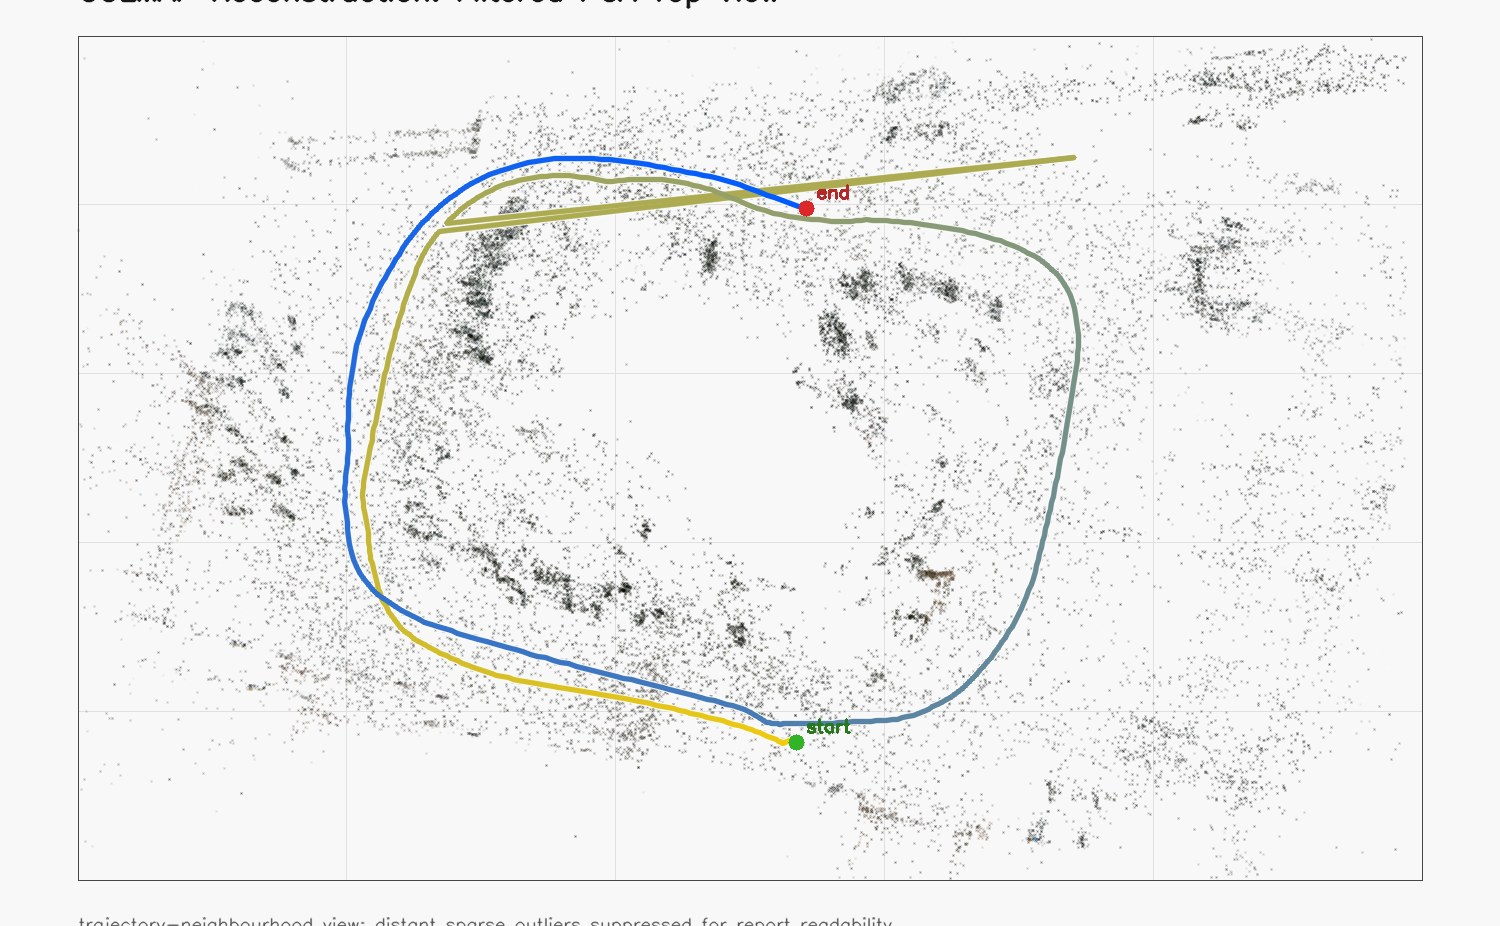
\includegraphics[width=0.24\textwidth]{images/Q2/figures/colmap/indoor_02/sparse_top_view.png}
}
\hfill
\subfloat[ORB-SLAM2 sparse top view.]{
    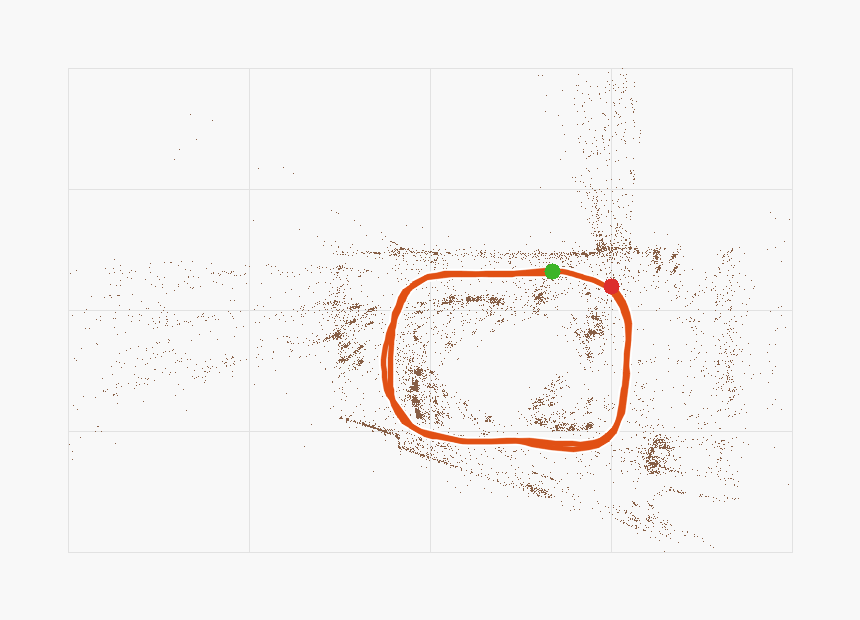
\includegraphics[width=0.24\textwidth]{images/Q2/figures/orbslam/indoor_02/indoor_map_top_view.png}
}
\hfill
\subfloat[EVO trajectory overlay.]{
    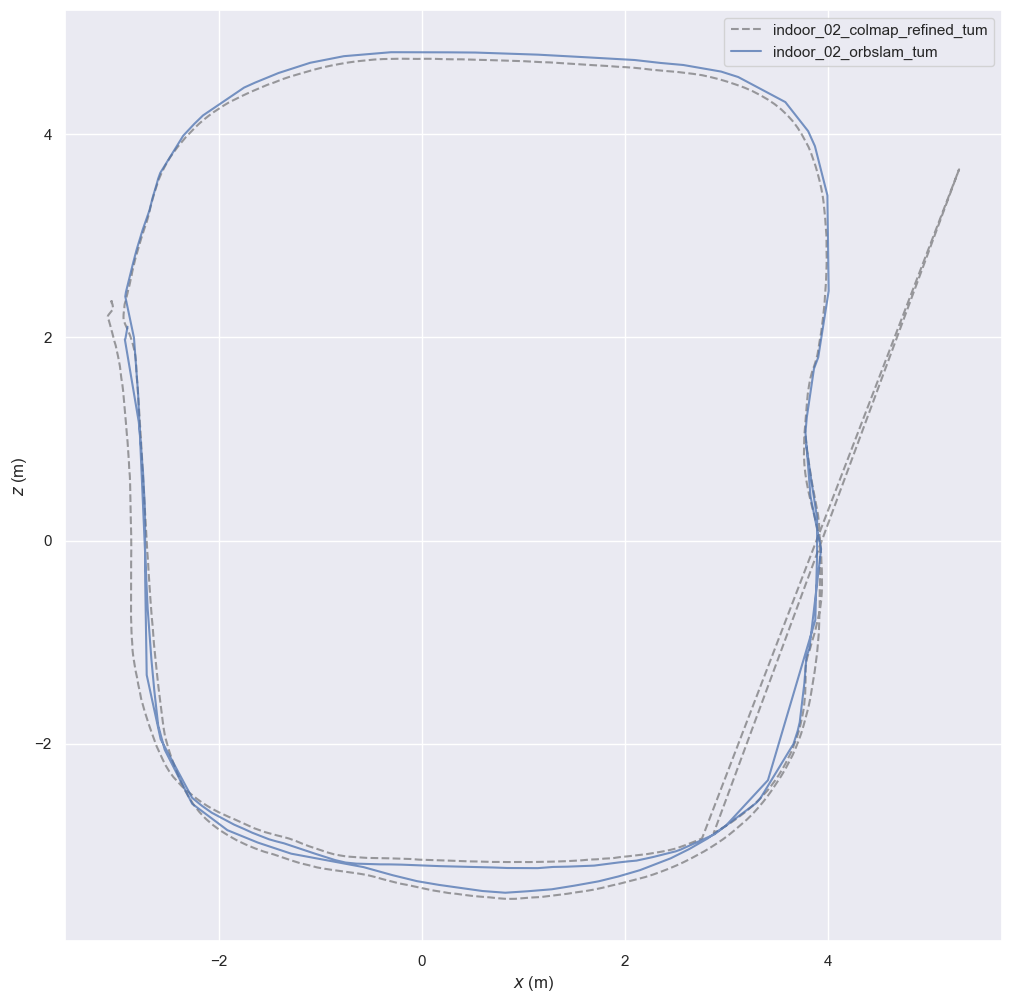
\includegraphics[width=0.24\textwidth]{images/Q2/figures/evo/indoor_02/trajectory_overlay.png}
}
\hfill
\subfloat[EVO APE map.]{
    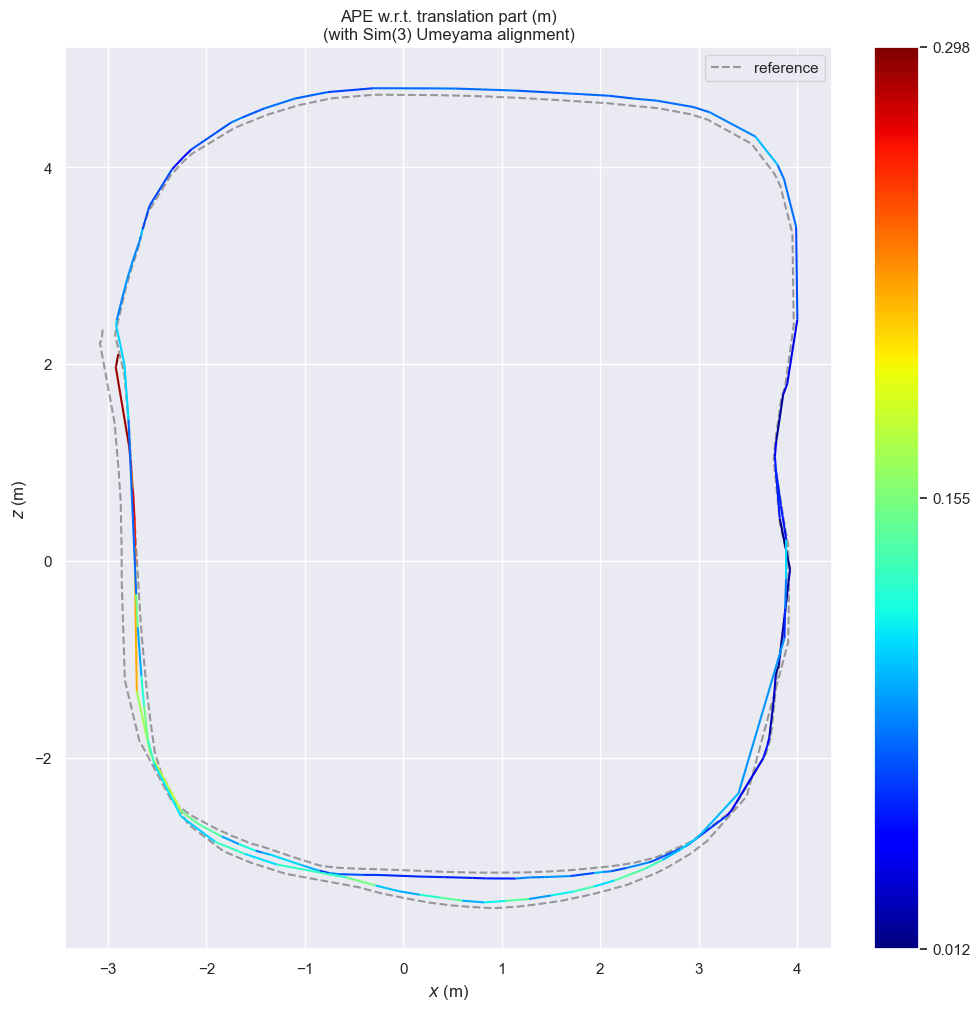
\includegraphics[width=0.24\textwidth]{images/Q2/figures/evo/indoor_02/ape_map.png}
}
\vspace{-1mm}
\caption{Indoor sequence results. COLMAP registered all sampled frames and recovered a loop-like trajectory, but the low-texture walls, glass, carpet, and repeated planar structure make this the harder sequence. ORB-SLAM2 also produced a coherent sparse map, while the EVO comparison shows larger local deviations than in the outdoor sequence.}
\label{fig:q2_indoor_summary}
\end{figure*}

\subsection{Outdoor Sequence}

The outdoor sequence produced a stronger reconstruction. COLMAP again registered all 600 sampled images, but the reconstruction contains more sparse points, more observations, longer tracks, and lower reprojection error than the indoor sequence. This matches the scene content: poles, barriers, signs, facade texture, and building edges provide more repeatable visual features.

Fig.~\ref{fig:q2_outdoor_summary} summarises the outdoor result. Although the sparse point cloud is not dense, the camera route is continuous and geometrically consistent with the acquisition path, which is sufficient for trajectory comparison. ORB-SLAM2 tracked the full outdoor stream and exported 179 keyframes with 12,979 sparse map points. After Sim(3) alignment, the ORB-SLAM2 trajectory closely follows the COLMAP trajectory over most of the route. The outdoor APE RMSE is 0.0298 and the RPE RMSE is 0.0204. Remaining errors occur mainly near turns and the end of the route, where feature overlap decreases and monocular drift becomes more visible.

\begin{figure*}[!t]
\centering
\subfloat[COLMAP sparse top view.]{
    
\includegraphics[width=0.24\textwidth]{images/Q2/figures/colmap/outdoor_01/sparse_top_view.png}
}
\hfill
\subfloat[ORB-SLAM2 sparse top view.]{
    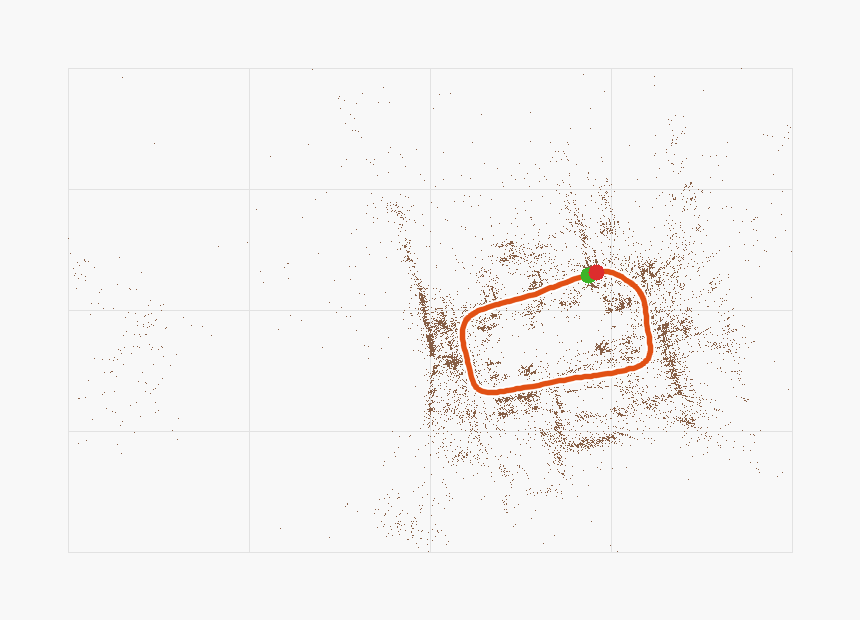
\includegraphics[width=0.24\textwidth]{images/Q2/figures/orbslam/outdoor_01/outdoor_map_top_view.png}
}
\hfill
\subfloat[EVO trajectory overlay.]{
    
\includegraphics[width=0.24\textwidth]{images/Q2/figures/evo/outdoor_01/trajectory_overlay.png}
}
\hfill
\subfloat[EVO APE map.]{
    
\includegraphics[width=0.24\textwidth]{images/Q2/figures/evo/outdoor_01/ape_map.png}
}
\vspace{-1mm}
\caption{Outdoor sequence results. The outdoor scene provides stronger geometric edges, poles, barriers, signs, and facade texture. This produces longer COLMAP tracks and more stable ORB-SLAM2 tracking. After Sim(3) alignment, the ORB-SLAM2 trajectory closely follows the COLMAP trajectory, with only small local errors near turns and the end of the route.}
\label{fig:q2_outdoor_summary}
\end{figure*}

\subsection{Quantitative Comparison}

Table~\ref{tab:q2_colmap_stats} summarises the COLMAP sparse reconstruction statistics. The outdoor sequence has 41,226 sparse points and a mean track length of 15.70, compared with 31,074 sparse points and 9.70 mean track length indoors. This supports the qualitative observation that the outdoor scene provides stronger and more persistent feature tracks.

\begin{table}[!t]
\caption{COLMAP sparse reconstruction statistics. Units are COLMAP reconstruction units because monocular scale is arbitrary.}
\centering
\footnotesize
\begin{tabular}{lcc}
\toprule
Quantity & Indoor & Outdoor \\
\midrule
Sampled images & 600 & 600 \\
Registered images & 600 & 600 \\
Sparse points & 31,074 & 41,226 \\
Observations & 301,296 & 647,183 \\
Mean track length & 9.70 & 15.70 \\
Mean reproj. error (px) & 0.673 & 0.538 \\
\bottomrule
\end{tabular}
\label{tab:q2_colmap_stats}
\end{table}

Table~\ref{tab:q2_evo_metrics} reports the EVO consistency metrics. These numbers measure agreement with COLMAP rather than absolute metric accuracy. The outdoor sequence has lower APE and RPE values, which is consistent with its sharper frames, stronger edges, more good matches, longer COLMAP tracks, and lower reprojection error.

\begin{table}[!t]
\caption{EVO consistency metrics after timestamp association and Sim(3) alignment to the refined COLMAP trajectory. Since no external ground truth was available, these values measure agreement with COLMAP rather than absolute metric accuracy.}
\centering
\footnotesize
\begin{tabular}{lcc}
\toprule
Metric & Indoor & Outdoor \\
\midrule
Synced ORB poses & 134 & 166 \\
APE RMSE & 0.1221 & 0.0298 \\
APE mean & 0.1045 & 0.0252 \\
APE max & 0.2979 & 0.1104 \\
RPE RMSE & 0.0281 & 0.0204 \\
RPE mean & 0.0229 & 0.0171 \\
RPE max & 0.0723 & 0.0480 \\
\bottomrule
\end{tabular}
\label{tab:q2_evo_metrics}
\end{table}

\subsection{Discussion and Limitations}

The indoor sequence remained valid, but it was harder for both COLMAP and ORB-SLAM2. The main causes were low-texture white walls, glass reflections, repeated planar layout, carpet, and occasional moving people. These factors reduce feature distinctiveness and make feature tracks shorter. ORB-SLAM2 is particularly sensitive to this because it is an online tracker that selects keyframes and map points incrementally.

The outdoor sequence showed closer agreement between ORB-SLAM2 and COLMAP. This should not be interpreted as absolute ground-truth accuracy. Instead, it indicates stronger consistency between two monocular pipelines after Sim(3) alignment. The improvement is explained by sharper frames, stronger geometric edges, more stable feature matches, longer COLMAP tracks, and lower reprojection error.

Several choices were important for stable results. Slow translational motion preserved feature overlap while still providing parallax. Using a single shared camera model in COLMAP avoided per-image intrinsics drift. Sampling every 3rd frame indoors and every 5th frame outdoors kept reconstruction tractable while preserving the full route. Increasing ORB-SLAM2 to 2000 ORB features helped retain enough landmarks in the indoor scene.

The evaluation is limited by the absence of external ground truth. Since both COLMAP and ORB-SLAM2 were used in monocular mode, absolute scale is not directly observable. Sim(3) alignment removes global scale differences, so the evaluation is suitable for comparing trajectory shape and local consistency, but not for claiming true metric accuracy.

The submitted video includes the raw indoor and outdoor streams, screen captures of ORB-SLAM2 reconstructing both scenes, COLMAP sparse reconstruction visualisations, and the EVO trajectory comparison plots. These materials provide supplementary evidence for the reconstruction quality and trajectory consistency discussed in this section.

\FloatBarrier

% ============================================================
\section{LiDAR SLAM with Our Own Sequences}
\label{sec:q3_lidar_slam}

% TODO: Insert Question 3 content here.
% Suggested structure:
% \subsection{Data Collection}
% \subsection{Laser Odometry and Mapping}
% \subsection{Maximum Range}
% \subsection{Angular Resolution}
% \subsection{Voxel Grid Downsampling}
% \subsection{Scan Rate}
% \subsection{Loop Closure Detection}
% \subsection{Factor Graph Optimisation}
% \subsection{Video Evidence and Discussion}

This section is reserved for Question 3. It should describe the three LiDAR sequences, point cloud maps, occupancy grid maps, robot trajectories, parameter analysis, loop closure detection, factor graph optimisation, and before/after loop closure comparison.

% ============================================================
\section{Conclusion}
\label{sec:conclusion}

% TODO: Add final group-level conclusion after Q1 and Q3 are inserted.

This report presents the group coursework results for visual and LiDAR SLAM. The final conclusion should summarise the main findings from the public visual SLAM experiments, the self-collected visual SLAM comparison, and the LiDAR SLAM mapping and optimisation experiments.

% ============================================================
% Optional bibliography placeholder. Add references if required.
% \begin{thebibliography}{00}
% \bibitem{orbslam2} R. Mur-Artal and J. D. Tardos, ``ORB-SLAM2: An Open-Source SLAM System for Monocular, Stereo, and RGB-D Cameras,'' IEEE Transactions on Robotics, 2017.
% \bibitem{colmap} J. L. Schonberger and J.-M. Frahm, ``Structure-from-Motion Revisited,'' CVPR, 2016.
% \end{thebibliography}

\end{document}